\documentclass[
  11pt,
  letterpaper,
   addpoints,
  answers
  ]{exam}

% Carga el preámbulo localizado en la carpeta superior
\NeedsTeXFormat{LaTeX2e}[2023/04/30]

% Provide the name of your page, the date it was last updated, and a comment about what it's used for
\ProvidesPackage{../exercise-preamble}[2023/04/30 Prof. Cassanelli custom LaTeX style]

% \usepackage{printlen}
% \uselengthunit{in}\printlength{\textwidth}

% PACKAGES
\usepackage[dvipsnames]{xcolor}

\usepackage{graphicx}
\graphicspath{{../figures}}
\usepackage{amsmath,amsthm,amssymb,mathtools,mathrsfs}
\usepackage{commath}
\usepackage{upgreek}
\usepackage{cancel}
\usepackage{enumerate}
\usepackage[font=small]{caption}
\usepackage[normalem]{ulem}
\usepackage{steinmetz}

\usepackage[left=1.5cm, right=1.5cm, top=1cm]{geometry}

% REFERENCES AND OTHERS
\usepackage{../aas_macros}
\usepackage{natbib}
\bibpunct{(}{)}{;}{a}{}{,}

\usepackage{tikz}
\usepackage{tikz-3dplot}
\usepackage{circuitikz}
\usepackage{pgfplots}
\pgfplotsset{compat=1.15}
\usepgfplotslibrary{smithchart}
\usetikzlibrary{
  decorations.pathmorphing,
  decorations.markings,
  calc,
  patterns,
  decorations,
  angles,
  quotes,
  ext.topaths.arcthrough,
  shapes
  }

\usepackage{siunitx}
\sisetup{
    range-phrase=\text{--},
    range-units=single,
    separate-uncertainty=true,
    print-unity-mantissa=false
    }
\DeclareSIUnit{\gauss}{G}
\DeclareSIUnit{\jansky}{Jy}

\newcommand{\iu}{\mathrm{i}\mkern1mu}
\newcommand{\ju}{\mathrm{j}\mkern1mu}
\newcommand{\euler}{\mathrm{e}}
\newcommand{\exponential}[1]{\mathrm{exp}\left[#1\right]}
\newcommand{\uvec}[1]{\widehat{\mathbf{#1}}}
\newcommand{\uvecs}[1]{\boldsymbol{\widehat{#1}}}
\newcommand{\bvec}[1]{\boldsymbol{\mathcal{#1}}}

\usepackage{hyperref}
\hypersetup{
    % bookmarks=true,
    unicode=true,
    pdftoolbar=true,
    pdfmenubar=true,
    pdffitwindow=false,
    pdfstartview={FitH},
    pdftitle={EL3103},
    pdfauthor={Tomas Cassanelli},
    pdfcreator={Tomas Cassanelli},
    pdfnewwindow=true,
    colorlinks=true,
    linkcolor=Violet,
    citecolor=Violet,
    urlcolor=Violet
    }

% Exam document class
\renewcommand{\figurename}{Figura}
\renewcommand{\tablename}{Cuadro}
\pagestyle{empty}

\usepackage[spanish]{cleveref}

\crefname{question}{\protect{pregunta}}{\protect{preguntas}}
\Crefname{question}{\protect{Pregunta}}{\protect{Preguntas}}
\creflabelformat{question}{#2{#1}#3}

\renewcommand{\solutiontitle}{\noindent\textbf{Solución:}\par\noindent}
\bracketedpoints
\pointname{~puntos}

\endinput

% Paquetes locales
\usepackage{float}
\usepackage{booktabs} % para \toprule, \midrule, \bottomrule
\usepackage{xcolor} % para colores
\usepackage{bm} % para negrita en símbolos matemáticos

% Macros locales
\newcommand{\Rel}{\mathfrak{R}} % símbolo para la reluctancia

\begin{document}

% Numeración de página
\pagestyle{plain}
\pagenumbering{arabic}

\noindent
\begin{minipage}{0.47\textwidth}
\includegraphics[width=\textwidth]{../fcfm_die}
\end{minipage}
\begin{minipage}{0.53\textwidth}
\begin{center} 
\large\textbf{Análisis de Sistemas Dinámicos y Estimación} (EL3204-1) \\
\large\textbf{Clase auxiliar 8} \\
\normalsize Prof.~ Marcos Orchard - Sebastián Espinosa.\\
\normalsize Prof.~Aux.~Erik Sáez
\end{center}
\end{minipage}

\vspace{0.5cm}
\noindent
\vspace{.85cm}
%----------------------------
\section{Resumen}

\subsubsection*{Variables Aleatorias}

Una \textbf{variable aleatoria} $X$ es una función que asigna un número real a cada resultado de un experimento aleatorio: $X : \Omega \longrightarrow \mathbb{R}$. En la práctica, trabajamos con las distribuciones de estas variables.\\

Las variables continuas tienen una \textbf{función de densidad de probabilidad} $f(x)$ que describe qué tan ``densa'' es la probabilidad alrededor de cada punto. No da probabilidades directas, sino que las probabilidades se calculan integrando: $\mathbb{P}(a \leq X \leq b) = \int_a^b f(x) \, dx$. Debe cumplir $f(x) \geq 0$ y $\int_{-\infty}^{\infty} f(x) \, dx = 1$.\\

Las variables discretas tienen una \textbf{función de probabilidad de masa} $p(x)$ que da directamente la probabilidad de cada valor específico. Debe cumplir $p(x) \geq 0$ y $\sum_{x} p(x) = 1$. Las probabilidades se calculan sumando: $\mathbb{P}(X \in A) = \sum_{x \in A} p(x)$.

\subsubsection*{Distribuciones Importantes}

\textbf{Distribución Uniforme} $X \sim U(a,b)$: Todos los valores en $[a,b]$ son igualmente probables.
\begin{equation}
f(x) = \begin{cases}
\frac{1}{b-a} & \text{si } x \in [a,b] \\
0 & \text{en otro caso}
\end{cases}
\end{equation}

\textbf{Distribución Exponencial} $X \sim \text{Exp}(\lambda)$: Modela tiempos de espera entre eventos. 
\begin{equation}
f(x) = \begin{cases}
\lambda e^{-\lambda x} & \text{si } x \geq 0 \\
0 & \text{en otro caso}
\end{cases}
\end{equation}

\textbf{Distribución Normal} $X \sim \mathcal{N}(\mu, \sigma^2)$: La distribución más importante. Curva en forma de campana.
\begin{equation}
f(x) = \frac{1}{\sqrt{2\pi}\sigma} \exp\left(-\frac{(x-\mu)^2}{2\sigma^2}\right)
\end{equation}
Propiedad clave: cualquier combinación lineal de variables normales independientes también es normal.

\textbf{Distribución Poisson} $X \sim \text{Poisson}(\lambda)$: Modela el número de eventos raros en un intervalo fijo.
\begin{equation}
p(x) = \begin{cases}
\frac{e^{-\lambda}\lambda^x}{x!} & \text{si } x \in \{0, 1, 2, \ldots\} \\
0 & \text{en otro caso}
\end{cases}
\end{equation}

\subsubsection*{Vectores Aleatorios}

Un \textbf{vector aleatorio} $\mathbf{X} = (X_1, X_2, \ldots, X_n)$ agrupa múltiples variables aleatorias. Su \textbf{función de densidad conjunta} describe el comportamiento conjunto:
\begin{equation}
f_{\mathbf{X}}(\mathbf{x}) = f_{X_1,X_2,\ldots,X_n}(x_1, x_2, \ldots, x_n)
\end{equation}

Para variables \textbf{independientes e idénticamente distribuidas (i.i.d.)}:
\begin{equation}
f_{\mathbf{X}}(\mathbf{x}) = \prod_{i=1}^n f_{X_i}(x_i)
\end{equation}

\subsubsection*{Momentos Estadísticos}

Los \textbf{momentos} caracterizan las propiedades de una distribución:

\textbf{Esperanza} (valor promedio esperado):
\begin{align}
\mathbb{E}[X] = \begin{cases}
\int_{-\infty}^{\infty} x \cdot f(x) \, dx & \text{si } X \text{ es continua} \\
\sum_x x \cdot p(x) & \text{si } X \text{ es discreta}
\end{cases}
\end{align}

\textbf{Varianza} (medida de dispersión):
\begin{equation}
\text{Var}(X) = \mathbb{E}[X^2] - (\mathbb{E}[X])^2
\end{equation}

\textbf{Covarianza} (dependencia lineal entre dos variables):
\begin{equation}
\text{Cov}(X,Y) = \mathbb{E}[XY] - \mathbb{E}[X]\mathbb{E}[Y]
\end{equation}

Para la distribución normal $X \sim \mathcal{N}(\mu, \sigma^2)$: $\mu = \mathbb{E}[X]$ y $\sigma^2 = \text{Var}(X)$.
\newpage
%----------------------------
\begin{questions}
  \question  
  
  Considere una variable aleatoria $X$ con distribución Poisson de parámetro $\lambda$.
  \begin{equation}
  P_X(X = k) = \frac{\lambda^k e^{-\lambda}}{k!},
  \end{equation}
  
  \begin{parts}
    \part Determine la función generadora de momentos de $X$, es decir:
    \begin{equation}
    M_X(t) = \sum_{k \geq 0} P_X(X = k) \cdot e^{tk},
    \end{equation}
    y verifique que es igual a $e^{\lambda(e^t - 1)}$.
    
    \part Considere $X_1, \ldots, X_n$ variables aleatorias independientes e idénticamente distribuidas (i.i.d.) con distribución Poisson de parámetro $\lambda$. Verifique que $X = \sum_{i=1}^n X_i$ es Poisson de parámetro $n\lambda$. \textit{Indicación:} Considere los resultados de probabilidades respecto a suma de variables aleatorias y las propiedades de la función generadora de momentos.
    
    \part Considere el problema de detección binario en el escenario paramétrico, donde $\Theta = \{0,1\}$ y se tiene que:
    \begin{align}
    \theta = 0 &\Rightarrow X \sim Poisson(\lambda_0), \\
    \theta = 1 &\Rightarrow X \sim Poisson(\lambda_1)
    \end{align}
    con $\lambda_1 > \lambda_0$. Determine la forma general de la familia de test óptimos dados por el Lema de Neyman-Pearson, y analice la forma de las zonas de decisión considerando que $\lambda_1 > \lambda_0$. Comente.
    
    \part Encuentre el test óptimo para el tamaño $\alpha = 0.01$. Considere $\lambda_0 = 2$ y $\lambda_1 = 4$. \textit{Indicación:} Notar que un test aleatorio podría ser necesario.
    
    \part Encuentre los valores de tamaño $\alpha$ sobre los cuales los test determinísticos son óptimos o en su defecto la condición que se debe cumplir para ello.
  \end{parts}
  %- ---------------------------
  \begin{solution}
      \subsection*{Resolución 1.1}
      
      La función generadora de momentos se define como:
      \begin{equation}
      M_X(t) = \mathbb{E}[e^{tX}] = \sum_{k=0}^{\infty} e^{tk} P_X(X = k)
      \end{equation}
      
      Sustituyendo la función de probabilidad de Poisson:
      \begin{align}
      M_X(t) &= \sum_{k=0}^{\infty} e^{tk} \cdot \frac{\lambda^k e^{-\lambda}}{k!} \\
      &= e^{-\lambda} \sum_{k=0}^{\infty} \frac{e^{tk} \lambda^k}{k!} \\
      &= e^{-\lambda} \sum_{k=0}^{\infty} \frac{(e^t \lambda)^k}{k!}
      \end{align}
      
      Reconocemos que la suma es la expansión en serie de Taylor de la función exponencial:
      \begin{equation}
      e^x = \sum_{k=0}^{\infty} \frac{x^k}{k!}
      \end{equation}
      
      Por lo tanto, con $x = e^t \lambda$:
      \begin{align}
      M_X(t) &= e^{-\lambda} \cdot e^{e^t \lambda} \\
      &= e^{-\lambda + e^t \lambda} \\
      &= e^{\lambda(e^t - 1)}
      \end{align}
      
      Con lo que se  demuestra que la función generadora de momentos de una variable Poisson con parámetro $\lambda$ es $M_X(t) = e^{\lambda(e^t - 1)}$.
      
      \subsection*{Resolución 1.2}

      Queremos demostrar que si $X_1, \ldots, X_n$ son variables aleatorias i.i.d. con distribución Poisson($\lambda$), entonces $X = \sum_{i=1}^n X_i \sim \text{Poisson}(n\lambda)$.

      La función generadora de momentos de la suma de variables independientes es el producto de sus funciones generadoras de momentos individuales:
      \begin{equation}
      M_X(t) = M_{\sum_{i=1}^n X_i}(t) = \prod_{i=1}^n M_{X_i}(t)
      \end{equation}
      
      Como cada $X_i \sim \text{Poisson}(\lambda)$, sabemos por la parte anterior que $M_{X_i}(t) = e^{\lambda(e^t - 1)}$. Por lo tanto:
      \begin{align}
      M_X(t) &= \prod_{i=1}^n e^{\lambda(e^t - 1)} \\
      &= \left[e^{\lambda(e^t - 1)}\right]^n \\
      &= e^{n\lambda(e^t - 1)}
      \end{align}
      
      Esta es exactamente la función generadora de momentos de una variable Poisson con parámetro $n\lambda$. Como la función generadora de momentos caracteriza únicamente la distribución, concluimos que:
      \begin{equation}
      X = \sum_{i=1}^n X_i \sim \text{Poisson}(n\lambda)
      \end{equation}

Con lo que podemos concluir que la suma de $n$ variables Poisson independientes con el mismo parámetro $\lambda$ es una variable Poisson con parámetro $n\lambda$. 

      \subsection*{Resolución 1.3}
      
      Consideremos un problema de detección binario donde debemos decidir entre dos hipótesis:
      \begin{align*}
      \mathcal{H}_0: \theta = 0 &\Rightarrow X \sim \text{Poisson}(\lambda_0) \\
      \mathcal{H}_1: \theta = 1 &\Rightarrow X \sim \text{Poisson}(\lambda_1)
      \end{align*}
      con $\lambda_1 > \lambda_0$.
      
      Para encontrar el test óptimo, aplicamos el Lema de Neyman-Pearson, que nos indica que debemos basar nuestra decisión en el cociente de verosimilitud:
      \begin{equation}
      L(x) = \frac{P_1(X = x)}{P_0(X = x)} = \frac{\frac{\lambda_1^x e^{-\lambda_1}}{x!}}{\frac{\lambda_0^x e^{-\lambda_0}}{x!}}
      \end{equation}
      
      Simplificando esta expresión, los factoriales se cancelan y obtenemos:
      \begin{align}
      L(x) &= \frac{\lambda_1^x e^{-\lambda_1}}{\lambda_0^x e^{-\lambda_0}} \\
      &= \left(\frac{\lambda_1}{\lambda_0}\right)^x \cdot e^{-(\lambda_1 - \lambda_0)}
      \end{align}
      
      Según el Lema de Neyman-Pearson, decidimos $\mathcal{H}_1$ cuando $L(x) > \eta$. Esto nos lleva a la condición:
      \begin{equation}
      \left(\frac{\lambda_1}{\lambda_0}\right)^x \cdot e^{-(\lambda_1 - \lambda_0)} > \eta
      \end{equation}
      
      Para simplificar esta desigualdad, tomamos logaritmo natural en ambos lados (recordando que el logaritmo es una función monótona creciente que preserva la desigualdad):
      \begin{align}
      x \ln\left(\frac{\lambda_1}{\lambda_0}\right) - (\lambda_1 - \lambda_0) &> \ln(\eta) \\
      x \ln\left(\frac{\lambda_1}{\lambda_0}\right) &> \ln(\eta) + (\lambda_1 - \lambda_0)
      \end{align}
      
      Ahora, dado que $\lambda_1 > \lambda_0$, tenemos que $\frac{\lambda_1}{\lambda_0} > 1$, lo que implica $\ln\left(\frac{\lambda_1}{\lambda_0}\right) > 0$. Por lo tanto, podemos dividir ambos lados por este logaritmo sin invertir la desigualdad:
      \begin{equation}
      x > \frac{\ln(\eta) + (\lambda_1 - \lambda_0)}{\ln\left(\frac{\lambda_1}{\lambda_0}\right)} = \gamma
      \end{equation}
      
      Con esto, la forma general del test óptimo queda definida como:
      \begin{equation}
      \pi(x) = \begin{cases}
      1 & \text{si } x > \gamma \quad \text{(decidir } \mathcal{H}_1\text{)} \\
      \gamma_0 & \text{si } x = \gamma \quad \text{(aleatorizar)} \\
      0 & \text{si } x < \gamma \quad \text{(decidir } \mathcal{H}_0\text{)}
      \end{cases}
      \end{equation}
      
      Los valores de $\gamma$ y $\gamma_0$ se eligen de manera que la probabilidad de falsa alarma sea exactamente igual a $\alpha$:
      \begin{equation}
      \mathbb{P}_{H_0}(\pi(X) = 1) = \alpha
      \end{equation}
      
      donde $\gamma_0$ representa el valor esperado (o probabilidad) de decidir $\mathcal{H}_1$ cuando $X = \gamma$, es decir, $\gamma_0 = \mathbb{E}[\pi(X) | X = \gamma]$. Notemos que aunque $\gamma_0$ toma valores en el intervalo $[0,1]$, en el contexto de detección binaria donde la decisión es 0 o 1, este valor representa la probabilidad de aleatorizar, permitiendo alcanzar cualquier tamaño $\alpha \in [0,1]$ (intervalo cerrado).
      
     El test óptimo tiene una estructura muy simple para distribuciones Poisson, siendo esencialmente un test de umbral sobre el número de eventos observados. La componente aleatoria (dada por $\gamma_0$) solo es necesaria cuando el umbral $\gamma$ cae exactamente en un valor entero y necesitamos ajustar con precisión la probabilidad de falsa alarma a exactamente $\alpha$.

      \subsection*{Resolución 1.4}
      
      Ahora debemos encontrar el test óptimo específico para $\alpha = 0.01$, con $\lambda_0 = 2$ y $\lambda_1 = 4$. Recordemos de la parte anterior que el test tiene la forma:
      \begin{equation}
      \pi(x) = \begin{cases}
      1 & \text{si } x > \gamma \\
      \gamma_0 & \text{si } x = \gamma \\
      0 & \text{si } x < \gamma
      \end{cases}
      \end{equation}
      
      donde debemos determinar $\gamma$ y $\gamma_0$ tal que la probabilidad de falsa alarma bajo $\mathcal{H}_0$ sea exactamente $\alpha = 0.01$:
      \begin{equation}
      \mathbb{P}_{H_0}(\pi(X) = 1) = \mathbb{P}_{H_0}(X > \gamma) + \gamma_0 \cdot \mathbb{P}_{H_0}(X = \gamma) = 0.01
      \end{equation}
      
      Bajo la hipótesis nula, $X \sim \text{Poisson}(2)$, por lo que debemos calcular las probabilidades acumuladas. Calculemos las probabilidades para distintos valores de $k$:
      
      \begin{align}
      P(X = k) &= \frac{2^k e^{-2}}{k!} \\
      P(X = 0) &= e^{-2} \approx 0.1353 \\
      P(X = 1) &= 2e^{-2} \approx 0.2707 \\
      P(X = 2) &= 2e^{-2} \approx 0.2707 \\
      P(X = 3) &= \frac{4e^{-2}}{3} \approx 0.1804 \\
      P(X = 4) &= \frac{2e^{-2}}{3} \approx 0.0902 \\
      P(X = 5) &= \frac{4e^{-2}}{15} \approx 0.0361 \\
      P(X = 6) &= \frac{4e^{-2}}{45} \approx 0.0120 \\
      P(X = 7) &= \frac{8e^{-2}}{315} \approx 0.0034
      \end{align}
      
      Ahora calculemos las probabilidades acumuladas de cola (tail probabilities):
      \begin{align}
      P(X \geq 6) &= P(X = 6) + P(X = 7) + \cdots \approx 0.0166 \\
      P(X \geq 7) &= P(X = 7) + P(X = 8) + \cdots \approx 0.0045
      \end{align}
      
      Observamos que $P(X \geq 7) \approx 0.0045 < 0.01 < 0.0166 \approx P(X \geq 6)$. Esto significa que un test determinístico puro no puede alcanzar exactamente $\alpha = 0.01$: si usamos $\gamma = 6$, tendríamos una probabilidad de falsa alarma de aproximadamente $0.0166 > 0.01$, mientras que si usamos $\gamma = 7$, tendríamos aproximadamente $0.0045 < 0.01$.
      
      Por lo tanto, necesitamos un test aleatorizado con $\gamma = 6$. Debemos encontrar $\gamma_0$ tal que:
      \begin{equation}
      P(X > 6) + \gamma_0 \cdot P(X = 6) = 0.01
      \end{equation}
      
      Despejando $\gamma_0$:
      \begin{align}
      \gamma_0 &= \frac{0.01 - P(X > 6)}{P(X = 6)} \\
      &= \frac{0.01 - P(X \geq 7)}{P(X = 6)} \\
      &= \frac{0.01 - 0.0045}{0.0120} \\
      &= \frac{0.0055}{0.0120} \\
      &\approx 0.458
      \end{align}
      
      Por lo tanto, el test óptimo en su versión aleatorizada es:
      \begin{equation}
      \pi(x) = \begin{cases}
      1 & \text{si } x \geq 7 \quad \text{(decidir } \mathcal{H}_1\text{)} \\
      0.458 & \text{si } x = 6 \quad \text{(valor esperado de la decisión)} \\
      0 & \text{si } x \leq 5 \quad \text{(decidir } \mathcal{H}_0\text{)}
      \end{cases}
      \end{equation}
      
      En la práctica, para implementar este test en detección binaria (donde solo podemos decidir 0 o 1), cuando observamos exactamente 6 eventos, aleatorizamos: lanzamos una moneda sesgada que con probabilidad 0.458 nos hace rechazar $\mathcal{H}_0$ (decidir 1) y con probabilidad 0.542 nos hace aceptarla (decidir 0). Si observamos 7 o más eventos, siempre rechazamos $\mathcal{H}_0$. Si observamos 5 o menos eventos, siempre aceptamos $\mathcal{H}_0$. Esta aleatorización es necesaria para alcanzar exactamente el nivel de significancia deseado de $\alpha = 0.01$.
      \subsection*{Resolución 1.5}
      
      Para determinar cuándo un test determinístico (sin aleatorización) es óptimo, debemos analizar la naturaleza discreta de la distribución Poisson y cómo esto afecta la construcción del test de Neyman-Pearson.
            
      Un test determinístico es óptimo cuando el tamaño $\alpha$ deseado coincide exactamente con una probabilidad acumulada de cola de la distribución bajo la hipótesis nula $\mathcal{H}_0$. Matemáticamente, esto ocurre cuando existe un entero $k^*$ tal que:
      \begin{equation}
      \alpha = \mathbb{P}_{H_0}(X \geq k^*) = \sum_{x = k^*}^{\infty} P_{H_0}(X = x)
      \end{equation}
      
      En este caso, el test óptimo determinístico tiene la forma simple:
      \begin{equation}
      \pi(x) = \begin{cases}
      1 & \text{si } x \geq k^* \quad \text{(rechazar } \mathcal{H}_0\text{)} \\
      0 & \text{si } x < k^* \quad \text{(aceptar } \mathcal{H}_0\text{)}
      \end{cases}
      \end{equation}
      
      y cumple exactamente $\mathbb{P}_{H_0}(\pi(X) = 1) = \alpha$ sin necesidad de aleatorización.
      
      Con $\lambda_0 = 2$ y $\lambda_1 = 4$, utilizando los cálculos de la parte anterior, las probabilidades de cola bajo $\mathcal{H}_0$ son:
      
      \begin{align*}
      \mathbb{P}_{H_0}(X \geq 4) &\approx 0.1429 \\
      \mathbb{P}_{H_0}(X \geq 5) &\approx 0.0527 \\
      \mathbb{P}_{H_0}(X \geq 6) &\approx 0.0166 \\
      \mathbb{P}_{H_0}(X \geq 7) &\approx 0.0045 \\
      \mathbb{P}_{H_0}(X \geq 8) &\approx 0.0011
      \end{align*}
      
      Por lo tanto, el test determinístico es óptimo para los siguientes valores de $\alpha$:
      \begin{equation}
      \alpha \in \{0.1429, 0.0527, 0.0166, 0.0045, 0.0011, \ldots\}
      \end{equation}
      Específicamente:
      
      \begin{itemize}
      \item Si $\alpha = 0.0166$, el test óptimo es determinístico con $k^* = 6$:
      \begin{equation}
      \pi(x) = \begin{cases}
      1 & \text{si } x \geq 6 \\
      0 & \text{si } x < 6
      \end{cases}
      \end{equation}
      
      \item Si $\alpha = 0.0045$, el test óptimo es determinístico con $k^* = 7$:
      \begin{equation}
      \pi(x) = \begin{cases}
      1 & \text{si } x \geq 7 \\
      0 & \text{si } x < 7
      \end{cases}
      \end{equation}
      
      \item Si $\alpha = 0.01$ (como en la parte 1.4), que está entre $0.0045$ y $0.0166$, \textbf{no} es posible un test determinístico óptimo, y se requiere aleatorización en $x = 6$.
      \end{itemize}
      
      Luego la condición necesaria y suficiente para que el test determinístico sea óptimo es:
      \begin{equation}
      \boxed{\alpha \in \left\{ \mathbb{P}_{H_0}(X \geq k) : k \in \mathbb{N} \right\}}
      \end{equation}
      
      Esta restricción es una consecuencia directa de la naturaleza discreta de la distribución Poisson. En distribuciones continuas, esta limitación no existe y siempre es posible encontrar un test determinístico para cualquier $\alpha \in (0,1)$. Para distribuciones discretas, cuando $\alpha$ no coincide con ninguna probabilidad de cola, la aleatorización es necesaria para alcanzar exactamente el nivel de significancia deseado, como se demostró en la parte 1.4. Sin embargo, con aleatorización es posible alcanzar cualquier tamaño $\alpha \in [0,1]$ (intervalo cerrado), incluyendo los extremos $\alpha = 0$ y $\alpha = 1$.
    \end{solution}
    %----------------------------
    \question
    Considere el problema clásico de comunicaciones digitales, de la detección de símbolos binarios contaminadas por ruido aditivo Gaussiano. En este caso $\Theta = \{0,1\}$ y la variable aleatoria de observación dado $\theta \in \Theta$ está dada por:
    \begin{equation}
    X = S_\theta + N
    \end{equation}
    con $S_0 = \mu$ y $S_1 = -\mu$, $\mu > 0$ y $N \sim \mathcal{N}(0, \sigma^2)$.
    
    Ahora asuma que se tienen múltiples mediciones (o en su defecto transmisiones sucesivas del mismo símbolo),
    \begin{equation}
    X_1, X_2, \ldots, X_n
    \end{equation}
    
    donde $X_i = S_\theta + N_i$ ($i = 1, \ldots, n$), para lo cual $N_1, \ldots, N_n$ son variables aleatorias i.i.d. que siguen una $\mathcal{N}(0, \sigma^2)$. Ahora la regla de decisión enfrenta el vector aleatorio Gaussiano $X_1^n = (X_1, \ldots, X_n)$ con valores en $\mathbb{R}^n$ y el espacio de decisión es $\Theta = \{0, 1\}$.
    
    \begin{parts}
        \part Condicionado a los valores de $\theta \in \Theta$, determine la distribución de $X_1^n$ y sus parámetros.
        
        \part Analice la familia de test óptimos y verifique que $\forall x_1^n \in \mathbb{R}^n$
        \begin{equation}
        \log\left( L(x_1^n) \right) = \frac{2}{\sigma^2} \bar{\mu}^T \cdot x_1^n
        \end{equation}
        
        donde $\bar{\mu} = (\mu, \mu, \ldots, \mu) \in \mathbb{R}^n$. Específicamente para $n = 2$ y $\eta = 0$, determine gráficamente las zonas de decisión, es decir:
        \begin{align}
        A_0 &= \pi_\eta^{-1}(\{0\}) = \left\{ x_1^2 \in \mathbb{R}^2 : \ln(L(x_1^2)) \leq \eta \right\}, \\
        A_1 &= \pi_\eta^{-1}(\{1\}) = \left\{ x_1^2 \in \mathbb{R}^2 : \ln(L(x_1^2)) > \eta \right\}.
        \end{align}
        
        \part Considere $\mu = 1$, $\sigma^2 = 10$ y $n = 1, 10, 10^2, 10^3$, respectivamente. Para estos distintos escenarios determine el test óptimo $\pi_\eta^* : \mathbb{R}^n \to \{0, 1\}$, tal que:
        \begin{equation}
        \alpha_\eta^* = \mathbb{E}(\pi_\eta^*(X_1^n) | \theta = 0) = 0.01
        \end{equation}
        
        y con ello grafique $\beta_\eta^* = \mathbb{E}(\pi_\eta^*(X_1^n) | \theta = 1)$ como función de $n$. Comente que observa en el poder del test y cuál es la influencia en el número de mediciones.
        
        \part Complemente el análisis anterior generando la curva ROC completa para los escenarios $n = 1, 10, 10^2, 10^3$. Comente en particular qué sucede cuando observado en el punto anterior.
    \end{parts}
    %----------------------------
    \begin{solution}
      \subsection*{Resolución 2.1}
      
      Necesitamos determinar la distribución conjunta del vector aleatorio $X_1^n = (X_1, X_2, \ldots, X_n)$ condicionado a cada valor de $\theta \in \Theta = \{0, 1\}$.
      
      Recordemos que cada observación tiene la forma:
      \begin{equation}
      X_i = S_\theta + N_i, \quad i = 1, 2, \ldots, n
      \end{equation}
      
      donde:
      \begin{itemize}
      \item $S_\theta$ es la señal transmitida que depende del símbolo $\theta$
      \item $N_i \sim \mathcal{N}(0, \sigma^2)$ son ruidos Gaussianos i.i.d.
      \end{itemize}
      
      Del enunciado del problema, sabemos que se trata de señalización antipodal es decir que:
      \begin{align}
      \theta = 0 &\Rightarrow S_0 = \mu \\
      \theta = 1 &\Rightarrow S_1 = -\mu
      \end{align}
      
    Luego debemos analizar por caso, por lo tanto cuando $\theta = 0$, tenemos $S_0 = \mu$, por lo tanto:
      \begin{equation}
      X_i = \mu + N_i \sim \mathcal{N}(\mu, \sigma^2)
      \end{equation}
      
      Como los $N_i$ son independientes e idénticamente distribuidos, las variables $X_1, X_2, \ldots, X_n$ son también independientes. Notemos que aunque los ruidos $N_i$ son i.i.d., cada observación $X_i$ tiene la misma señal determinística $\mu$ sumada al ruido. Esto significa que:
      \begin{itemize}
      \item Cada $X_i$ tiene la misma distribución marginal: $X_i \sim \mathcal{N}(\mu, \sigma^2)$ (idénticamente distribuidas)
      \item Las observaciones $X_1, \ldots, X_n$ son independientes entre sí (debido a la independencia de los ruidos $N_i$)
      \end{itemize}
      
      Por lo tanto, el vector aleatorio $X_1^n = (X_1, X_2, \ldots, X_n)$ sigue una distribución normal multivariada:
      \begin{equation}
      X_1^n | \theta = 0 \sim \mathcal{N}(\bar{\mu}, \sigma^2 I_n)
      \end{equation}
      
      donde:
      \begin{itemize}
      \item $\bar{\mu} = (\mu, \mu, \ldots, \mu)^T \in \mathbb{R}^n$ es el vector de medias. Cada componente es $\mu$ porque cada observación $X_i$ tiene esperanza $\mathbb{E}[X_i] = \mathbb{E}[\mu + N_i] = \mu + \mathbb{E}[N_i] = \mu$. Como todas las observaciones tienen la misma media, obtenemos un vector con componentes iguales.
      
      \item $\sigma^2 I_n$ es la matriz de covarianza, con $I_n$ siendo la matriz identidad de dimensión $n \times n$. La forma diagonal refleja la independencia de las observaciones: $\text{Cov}(X_i, X_j) = 0$ para $i \neq j$, y $\text{Var}(X_i) = \sigma^2$ para todo $i$.
      \end{itemize}
      
      En otras palabras, trabajamos con un vector porque tenemos $n$ observaciones simultáneas, y aunque cada una tiene la misma distribución marginal (i.i.d.), necesitamos considerar su distribución conjunta para el test óptimo. El vector de medias tiene todas sus componentes iguales a $\mu$ precisamente porque cada medición observa la misma señal $\mu$ contaminada por ruido independiente.
      
      La función de densidad de probabilidad conjunta es:
      \begin{equation}
      f_0(x_1^n) = \prod_{i=1}^n \frac{1}{\sqrt{2\pi\sigma^2}} \exp\left(-\frac{(x_i - \mu)^2}{2\sigma^2}\right) = \frac{1}{(2\pi\sigma^2)^{n/2}} \exp\left(-\frac{1}{2\sigma^2}\sum_{i=1}^n (x_i - \mu)^2\right)
      \end{equation}
      
      o en forma vectorial:
      \begin{equation}
      f_0(x_1^n) = \frac{1}{(2\pi\sigma^2)^{n/2}} \exp\left(-\frac{\|x_1^n - \bar{\mu}\|^2}{2\sigma^2}\right)
      \end{equation}
      
      
      Por otro lado cuando $\theta = 1$, tenemos $S_1 = -\mu$, por lo tanto:
      \begin{equation}
      X_i = -\mu + N_i \sim \mathcal{N}(-\mu, \sigma^2)
      \end{equation}
      
      Nuevamente, por la independencia de los $N_i$, el vector aleatorio $X_1^n$ sigue una distribución normal multivariada:
      \begin{equation}
      X_1^n | \theta = 1 \sim \mathcal{N}(-\bar{\mu}, \sigma^2 I_n)
      \end{equation}
      
      donde:
      \begin{itemize}
      \item $-\bar{\mu} = (-\mu, -\mu, \ldots, -\mu)^T \in \mathbb{R}^n$ es el vector de medias
      \item $\sigma^2 I_n$ es la matriz de covarianza (la misma que en el caso $\theta = 0$)
      \end{itemize}
      
      La función de densidad de probabilidad conjunta es:
      \begin{equation}
      f_1(x_1^n) = \prod_{i=1}^n \frac{1}{\sqrt{2\pi\sigma^2}} \exp\left(-\frac{(x_i + \mu)^2}{2\sigma^2}\right) = \frac{1}{(2\pi\sigma^2)^{n/2}} \exp\left(-\frac{1}{2\sigma^2}\sum_{i=1}^n (x_i + \mu)^2\right)
      \end{equation}
      
      o en forma vectorial:
      \begin{equation}
      f_1(x_1^n) = \frac{1}{(2\pi\sigma^2)^{n/2}} \exp\left(-\frac{\|x_1^n + \bar{\mu}\|^2}{2\sigma^2}\right)
      \end{equation}
    
      
Luego el vector aleatorio $X_1^n$ tiene las siguientes distribuciones condicionadas bajo señalización antipodal:
      \begin{align}
      \theta = 0 &\Rightarrow X_1^n \sim \mathcal{N}\left(\bar{\mu}, \sigma^2 I_n\right) \\
      \theta = 1 &\Rightarrow X_1^n \sim \mathcal{N}\left(-\bar{\mu}, \sigma^2 I_n\right)
      \end{align}
      
      donde $\bar{\mu} = (\mu, \mu, \ldots, \mu)^T$ y las matrices de covarianza son idénticas en ambos casos debido a que el ruido tiene la misma varianza independientemente del símbolo transmitido. 
      
      \subsection*{Resolución 2.2}
      
      Para aplicar el Lema de Neyman-Pearson, necesitamos calcular el cociente de verosimilitud el cual viene dadao por:
      \begin{equation}
      L(x_1^n) = \frac{f_1(x_1^n)}{f_0(x_1^n)}
      \end{equation}
      
      Sustituyendo las densidades obtenidas en la parte anterior (señalización antipodal):
      \begin{align}
      L(x_1^n) &= \frac{\frac{1}{(2\pi\sigma^2)^{n/2}} \exp\left(-\frac{\|x_1^n + \bar{\mu}\|^2}{2\sigma^2}\right)}{\frac{1}{(2\pi\sigma^2)^{n/2}} \exp\left(-\frac{\|x_1^n - \bar{\mu}\|^2}{2\sigma^2}\right)} \\
      &= \frac{\exp\left(-\frac{\|x_1^n + \bar{\mu}\|^2}{2\sigma^2}\right)}{\exp\left(-\frac{\|x_1^n - \bar{\mu}\|^2}{2\sigma^2}\right)} \\
      &= \exp\left(\frac{\|x_1^n - \bar{\mu}\|^2 - \|x_1^n + \bar{\mu}\|^2}{2\sigma^2}\right)
      \end{align}
      
      Desarrollemos el término en el exponente. Tenemos:
      \begin{align}
      \|x_1^n - \bar{\mu}\|^2 &= \sum_{i=1}^n (x_i - \mu)^2 = \sum_{i=1}^n x_i^2 - 2\mu \sum_{i=1}^n x_i + n\mu^2 \\
      \|x_1^n + \bar{\mu}\|^2 &= \sum_{i=1}^n (x_i + \mu)^2 = \sum_{i=1}^n x_i^2 + 2\mu \sum_{i=1}^n x_i + n\mu^2
      \end{align}
      
      Por lo tanto:
      \begin{align}
      \|x_1^n - \bar{\mu}\|^2 - \|x_1^n + \bar{\mu}\|^2 &= \left(\sum_{i=1}^n x_i^2 - 2\mu \sum_{i=1}^n x_i + n\mu^2\right) - \left(\sum_{i=1}^n x_i^2 + 2\mu \sum_{i=1}^n x_i + n\mu^2\right) \\
      &= -4\mu \sum_{i=1}^n x_i \\
      &= -4\mu \bar{\mu}^T \cdot x_1^n / \mu \\
      &= -4 \bar{\mu}^T \cdot x_1^n
      \end{align}
      
      Sustituyendo en la expresión del cociente de verosimilitud:
      \begin{equation}
      L(x_1^n) = \exp\left(\frac{-4 \bar{\mu}^T \cdot x_1^n}{2\sigma^2}\right) = \exp\left(\frac{-2 \bar{\mu}^T \cdot x_1^n}{\sigma^2}\right)
      \end{equation}
      
      Tomando logaritmo natural del cociente de verosimilitud $L(x_1^n)$:
      \begin{equation}
      \boxed{\log(L(x_1^n)) = \frac{-2}{\sigma^2} \bar{\mu}^T \cdot x_1^n}
      \end{equation}
      
      donde $L(x_1^n)$ es el cociente de verosimilitud (likelihood ratio en inglés).
      
      Con lo cual se cumple lo pedido. Ahora determinamos las zonas de decisión para $n=2$ y $\eta=0$. Para $n=2$, tenemos $x_1^2 = (x_1, x_2)$ y $\bar{\mu} = (\mu, \mu)$. El logaritmo del cociente de verosimilitud es:
      \begin{equation}
      \log(L(x_1, x_2)) = \frac{-2}{\sigma^2} \mu(x_1 + x_2)
      \end{equation}
      
      Con $\eta = 0$, la regla de decisión es:
      \begin{equation}
      \log(L(x_1, x_2)) > 0 \quad \Rightarrow \quad \frac{-2}{\sigma^2} \mu(x_1 + x_2) > 0
      \end{equation}
      
      Dado que $\mu > 0$ y $\sigma^2 > 0$, esto se simplifica a:
      \begin{equation}
      x_1 + x_2 < 0
      \end{equation}
      
      Por lo tanto, las zonas de decisión son:
      \begin{align}
      A_0 &= \left\{ (x_1, x_2) \in \mathbb{R}^2 : x_1 + x_2 \geq 0 \right\} \quad \text{(Decidir } \mathcal{H}_0: S_0 = \mu\text{)} \\
      A_1 &= \left\{ (x_1, x_2) \in \mathbb{R}^2 : x_1 + x_2 < 0 \right\} \quad \text{(Decidir } \mathcal{H}_1: S_1 = -\mu\text{)}
      \end{align}
      
      \textbf{Observación importante}: En este caso de señalización antipodal con distribuciones Gaussianas, la familia de test óptimos es completamente determinística (sin necesidad de aleatorización). Esto se debe a que la variable aleatoria inducida por el estadístico es absolutamente continua, lo que permite alcanzar cualquier tamaño $\alpha \in [0,1]$ mediante la elección apropiada del umbral $\eta$, sin requerir aleatorización como en el caso discreto (Poisson).
      
      En el plano $(x_1, x_2)$, la frontera de decisión es la recta $x_1 + x_2 = 0$ (la diagonal que pasa por el origen). Esta recta divide el plano en dos semiplanos:
      \begin{itemize}
      \item \textbf{Región $A_0$} (azul): Semiplano donde $x_1 + x_2 \geq 0$ (primer y cuarto cuadrante más el eje positivo), decidimos $\mathcal{H}_0$, es decir, símbolo $+\mu$
      \item \textbf{Región $A_1$} (roja): Semiplano donde $x_1 + x_2 < 0$ (segundo y tercer cuadrante más el eje negativo), decidimos $\mathcal{H}_1$, es decir, símbolo $-\mu$
      \end{itemize}
      
      La frontera de decisión es una recta con pendiente $-1$ que pasa por el origen. Esto tiene perfecto sentido para señalización antipodal:
      \begin{itemize}
      \item Si las observaciones $x_1$ y $x_2$ son en promedio positivas ($x_1 + x_2 > 0$), es más probable que el símbolo transmitido haya sido $+\mu$ (hipótesis $\mathcal{H}_0$)
      \item Si las observaciones son en promedio negativas ($x_1 + x_2 < 0$), es más probable que el símbolo transmitido haya sido $-\mu$ (hipótesis $\mathcal{H}_1$)
      \end{itemize}
      
    
      \begin{figure}[H]
      \centering
      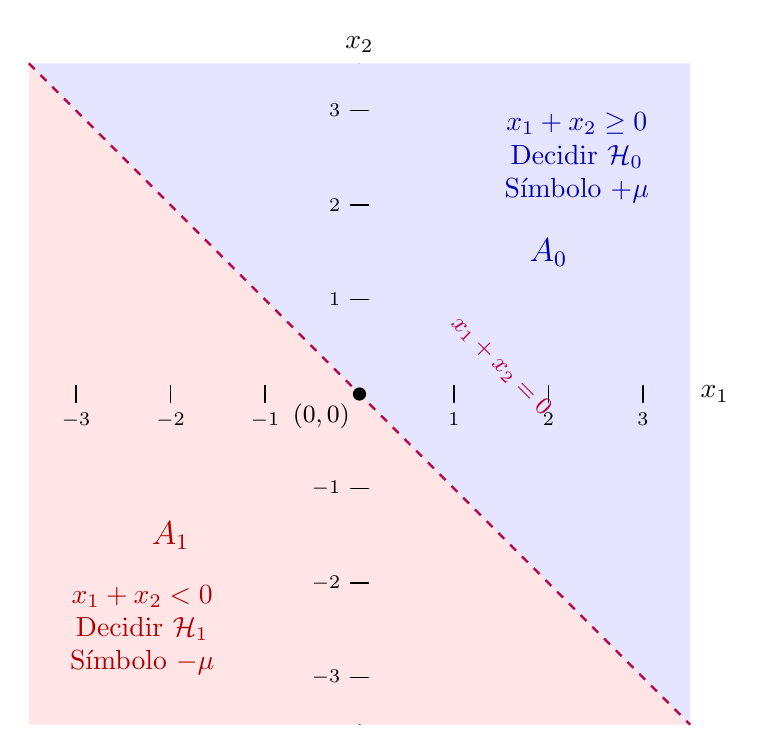
\begin{tikzpicture}[scale=1.2]
      % Ejes
      \draw[->, thick] (-3.5,0) -- (3.5,0) node[right] {$x_1$};
      \draw[->, thick] (0,-3.5) -- (0,3.5) node[above] {$x_2$};
      
      % Regiones de decisión (sombreadas)
      % Región azul A_0: donde x_1 + x_2 >= 0 (arriba/derecha de la diagonal)
      \fill[blue!10] (-3.5,3.5) -- (3.5,3.5) -- (3.5,-3.5) -- (-3.5,3.5) -- cycle;
      % Región roja A_1: donde x_1 + x_2 < 0 (abajo/izquierda de la diagonal)
      \fill[red!10] (-3.5,-3.5) -- (3.5,-3.5) -- (-3.5,3.5) -- cycle;
      
      % Frontera de decisión
      \draw[thick, purple, dashed] (-3.5,3.5) -- (3.5,-3.5);
      
      % Etiquetas de regiones
      \node[blue!70!black, font=\large\bfseries] at (2,1.5) {$A_0$};
      \node[red!70!black, font=\large\bfseries] at (-2,-1.5) {$A_1$};
      
      % Anotaciones
      \node[blue!70!black, align=center] at (2.3,2.5) {$x_1 + x_2 \geq 0$\\Decidir $\mathcal{H}_0$\\Símbolo $+\mu$};
      \node[red!70!black, align=center] at (-2.3,-2.5) {$x_1 + x_2 < 0$\\Decidir $\mathcal{H}_1$\\Símbolo $-\mu$};
      
      % Etiqueta de frontera
      \node[purple, font=\small, rotate=-45] at (1.5,0.3) {$x_1 + x_2 = 0$};
      
      % Punto origen
      \fill[black] (0,0) circle (2pt);
      \node[below left, font=\small] at (0,0) {$(0,0)$};
      
      % Marcas en los ejes
      \foreach \x in {-3,-2,-1,1,2,3}
      \draw (\x,0.1) -- (\x,-0.1) node[below, font=\scriptsize] {$\x$};
      \foreach \y in {-3,-2,-1,1,2,3}
      \draw (0.1,\y) -- (-0.1,\y) node[left, font=\scriptsize] {$\y$};
      
      \end{tikzpicture}
      \caption{Regiones de decisión en el plano $(x_1, x_2)$ para señalización antipodal con $n=2$ y $\eta=0$. La frontera de decisión $x_1 + x_2 = 0$ divide el plano en dos semiplanos: la región $A_0$ (azul) donde se decide el símbolo $+\mu$, y la región $A_1$ (roja) donde se decide el símbolo $-\mu$.}
      \label{fig:regiones_decision_antipodal}
      \end{figure}
      
      \subsection*{Resolución 2.3}
      
      Para resolver esta parte, necesitamos determinar el test óptimo para cada valor de $n$ tal que la probabilidad de falsa alarma sea $\alpha = 0.01$, y luego calcular la potencia del test (probabilidad de detección correcta) $\beta_\eta^*$.
      
      \textbf{Construcción del test óptimo con señalización antipodal:}
      
      Del análisis anterior, sabemos que un estadístico suficiente (función de las observaciones que resume toda la información relevante para la decisión) es:
      \begin{equation}
      T(X_1^n) = \sum_{i=1}^n X_i
      \end{equation}
      
      Bajo la hipótesis nula ($\theta = 0$, símbolo $+\mu$):
      \begin{equation}
      T(X_1^n) | \theta = 0 = \sum_{i=1}^n (\mu + N_i) = n\mu + \sum_{i=1}^n N_i \sim \mathcal{N}(n\mu, n\sigma^2)
      \end{equation}
      
      Bajo la hipótesis alternativa ($\theta = 1$, símbolo $-\mu$):
      \begin{equation}
      T(X_1^n) | \theta = 1 = \sum_{i=1}^n (-\mu + N_i) = -n\mu + \sum_{i=1}^n N_i \sim \mathcal{N}(-n\mu, n\sigma^2)
      \end{equation}
      
      La regla de decisión óptima para señalización antipodal es:
      \begin{equation}
      \text{Decidir } \mathcal{H}_1 \text{ si } T(X_1^n) < \gamma
      \end{equation}
      
      Es decir, decidimos el símbolo $-\mu$ cuando la suma es suficientemente negativa. Notemos que con umbral en cero ($\gamma = 0$), obtenemos una regla de decisión simétrica que es natural para señales antipodales.
      
      Para analizar con $\alpha = 0.01$, necesitamos encontrar $\gamma$ tal que:
      \begin{equation}
      \mathbb{P}_{H_0}(T(X_1^n) < \gamma) = \alpha = 0.01
      \end{equation}
      
      Estandarizando bajo $\mathcal{H}_0$:
      \begin{equation}
      \mathbb{P}_{H_0}\left(\frac{T(X_1^n) - n\mu}{\sqrt{n\sigma^2}} < \frac{\gamma - n\mu}{\sqrt{n\sigma^2}}\right) = \alpha
      \end{equation}
      
      Si $Z \sim \mathcal{N}(0,1)$, entonces:
      \begin{equation}
      \mathbb{P}(Z < -z_\alpha) = \alpha \quad \Rightarrow \quad \frac{\gamma - n\mu}{\sigma\sqrt{n}} = -z_\alpha
      \end{equation}
      
      Para $\alpha = 0.01$, tenemos $z_{0.01} \approx 2.326$. Por lo tanto:
      \begin{equation}
      \gamma = n\mu - z_\alpha \sigma \sqrt{n}
      \end{equation}
      
      
      La probabilidad de detección correcta es:
      \begin{align}
      \beta_\eta^* &= \mathbb{P}_{H_1}(T(X_1^n) < \gamma) \\
      &= \mathbb{P}_{H_1}\left(\frac{T(X_1^n) + n\mu}{\sqrt{n\sigma^2}} < \frac{\gamma + n\mu}{\sqrt{n\sigma^2}}\right) \\
      &= \mathbb{P}\left(Z < \frac{n\mu - z_\alpha \sigma\sqrt{n} + n\mu}{\sigma\sqrt{n}}\right) \\
      &= \mathbb{P}\left(Z < \frac{2n\mu - z_\alpha \sigma\sqrt{n}}{\sigma\sqrt{n}}\right) \\
      &= \mathbb{P}\left(Z < \frac{2\mu\sqrt{n}}{\sigma} - z_\alpha\right) \\
      &= \Phi\left(\frac{2\mu\sqrt{n}}{\sigma} - z_\alpha\right)
      \end{align}
      
      donde en el último paso hemos introducido la notación $\Phi(\cdot)$ para la función de distribución acumulada (CDF) de la normal estándar:
      \begin{equation}
      \Phi(x) = \mathbb{P}(Z \leq x) = \int_{-\infty}^x \frac{1}{\sqrt{2\pi}} e^{-t^2/2} \, dt
      \end{equation}

      Esta función $\Phi$ nos permite expresar probabilidades de la forma $\mathbb{P}(Z < x)$ de manera compacta. El cambio de notación de $\mathbb{P}(Z < x)$ a $\Phi(x)$ es simplemente una convención: ambas representan exactamente lo mismo, pero $\Phi$ es más conveniente cuando trabajamos con la distribución normal estándar repetidamente. Es importante notar que $\Phi$ es una función conocida y tabulada (o implementada en software estadístico), lo que nos permite calcular numéricamente la potencia del test para cualquier valor de $n$.
      
      \textbf{Cálculo numérico para los valores dados:}

      
      Con $\mu = 1$, $\sigma^2 = 10$ (por lo tanto $\sigma = \sqrt{10} \approx 3.162$), y $z_{0.01} \approx 2.326$:
      
      \begin{align}
      n = 1: \quad & \beta^* = \Phi\left(\frac{2 \cdot 1 \cdot 1}{3.162} - 2.326\right) = \Phi(-1.694) \approx 0.045 \\
      n = 10: \quad & \beta^* = \Phi\left(\frac{2 \cdot 1 \cdot \sqrt{10}}{3.162} - 2.326\right) = \Phi(-0.326) \approx 0.372 \\
      n = 100: \quad & \beta^* = \Phi\left(\frac{2 \cdot 1 \cdot 10}{3.162} - 2.326\right) = \Phi(3.999) \approx 1.000 \\
      n = 1000: \quad & \beta^* = \Phi\left(\frac{2 \cdot 1 \cdot \sqrt{1000}}{3.162} - 2.326\right) = \Phi(17.674) \approx 1.000
      \end{align}
      
  Algunos aspectos importantes a destacar:
      
      \begin{itemize}
      \item \textbf{Efecto del número de mediciones:} La potencia del test $\beta^*$ aumenta significativamente con el número de mediciones $n$. Con una sola medición ($n=1$), la potencia es apenas $4.5\%$. Con $n=10$ mediciones, la potencia aumenta a $37.2\%$. Con $n=100$ mediciones, la potencia es prácticamente $100\%$.
      
      \item \textbf{Ventaja de la señalización antipodal:} Comparado con señalización ON-OFF (donde un símbolo es cero), la señalización antipodal aprovecha mejor la energía disponible, ya que ambos símbolos están a distancia $\mu$ del origen. La distancia efectiva entre símbolos es $2\mu$, lo que duplica la capacidad de discriminación.
      
      \item \textbf{Relación con $\sqrt{n}$:} La potencia mejora con $\sqrt{n}$ debido a que la varianza del promedio decrece como $1/n$, mientras que la diferencia entre medias escala con $n$.
      

      \end{itemize}
      
      \subsection*{Resolución 2.4}
      
      Para generar la curva ROC completa, debemos analizar cómo varía la potencia del test $\beta$ (probabilidad de detección) en función del tamaño del test $\alpha$ (probabilidad de falsa alarma) para diferentes valores de $n$.
      
      
      La curva ROC se construye graficando $\beta(\alpha)$ versus $\alpha$ para $\alpha \in [0,1]$. Del análisis anterior, sabemos que:
      
      Para un tamaño de test $\alpha$ dado, el umbral es:
      \begin{equation}
      \gamma = n\mu - z_\alpha \sigma \sqrt{n}
      \end{equation}
      
      donde $z_\alpha = \Phi^{-1}(1-\alpha)$ es el cuantil de la distribución normal estándar tal que $\mathbb{P}(Z < -z_\alpha) = \alpha$. La potencia del test correspondiente es:
      \begin{equation}
      \beta(\alpha) = \mathbb{P}_{H_1}(T(X_1^n) < \gamma) = \Phi\left(\frac{2\mu\sqrt{n}}{\sigma} - z_\alpha\right)
      \end{equation}
      
      Sustituyendo $z_\alpha = \Phi^{-1}(1-\alpha)$:
      \begin{equation}
      \beta(\alpha) = \Phi\left(\frac{2\mu\sqrt{n}}{\sigma} - \Phi^{-1}(1-\alpha)\right)
      \end{equation}
      
      o equivalentemente:
      \begin{equation}
      \beta(\alpha) = \Phi\left(\Phi^{-1}(\alpha) + \frac{2\mu\sqrt{n}}{\sigma}\right)
      \end{equation}
      
      
      La curva ROC tiene las siguientes propiedades importantes:
      
      \begin{itemize}
      \item \textbf{Punto (0,0):} Corresponde a un test que nunca rechaza $\mathcal{H}_0$ (decisión trivial: siempre aceptar $\mathcal{H}_0$). Se tiene $\alpha = 0$ y $\beta = 0$.
      
      \item \textbf{Punto (1,1):} Corresponde a un test que siempre rechaza $\mathcal{H}_0$ (decisión trivial: siempre decidir $\mathcal{H}_1$). Se tiene $\alpha = 1$ y $\beta = 1$.
      
      \item \textbf{Diagonal $\beta = \alpha$:} Representa un test aleatorio sin información (equivalente a lanzar una moneda). Un buen test debe estar por encima de esta diagonal.
      
      \item \textbf{Punto de operación anterior ($\alpha = 0.01$):} Este es el punto específico analizado en la parte 2.3, donde fijamos $\alpha = 0.01$ y calculamos los valores de $\beta$ correspondientes.
      \end{itemize}
      
      A continuación, se presentan las curvas ROC para los diferentes valores de $n$ (1, 10, 100, 1000) con $\mu = 1$ y $\sigma^2 = 10$. Cada curva se genera variando $\alpha$ desde 0 hasta 1 y calculando el correspondiente $\beta(\alpha)$.
      
      \begin{enumerate}
      \item \textbf{$n = 1$:}
      
      Con una sola medición en señalización antipodal, la curva ROC muestra una capacidad de discriminación limitada pero mejor que el caso unipolar. Para $\alpha = 0.01$, obtuvimos $\beta \approx 0.045$, lo que significa que la probabilidad de detectar correctamente el símbolo $-\mu$ es del 4.5\%.
      
      El área bajo la curva (AUC) para este caso es aproximadamente 0.58, indicando rendimiento modesto pero mejor que el azar.
      
      \item \textbf{$n = 10$:}
      
      Con 10 mediciones, la curva ROC se aleja notablemente de la diagonal. Para $\alpha = 0.01$, tenemos $\beta \approx 0.372$, mejorando significativamente la capacidad de detección. El AUC aumenta considerablemente a aproximadamente 0.79.
      
      \item \textbf{$n = 100$:}
      
      Con 100 mediciones, la curva ROC se acerca mucho a la esquina superior izquierda (punto ideal (0,1)). Para $\alpha = 0.01$, tenemos $\beta \approx 1.000$, lo que significa que podemos detectar la señal con probabilidad casi perfecta manteniendo una tasa de falsa alarma muy baja.
      
      El AUC es mayor a 0.99, indicando un excelente rendimiento.
      
      \item \textbf{$n = 1000$:}
      
      Con 1000 mediciones, la curva ROC es prácticamente una línea que va de (0,0) a (0,1) y luego a (1,1), siguiendo el eje vertical y luego el horizontal. Para $\alpha = 0.01$, tenemos $\beta \approx 1.0$, lo que significa detección perfecta.
      
      El AUC es prácticamente 1, indicando rendimiento perfecto.
      \end{enumerate}
    
      
      \begin{figure}[H]
      \centering
      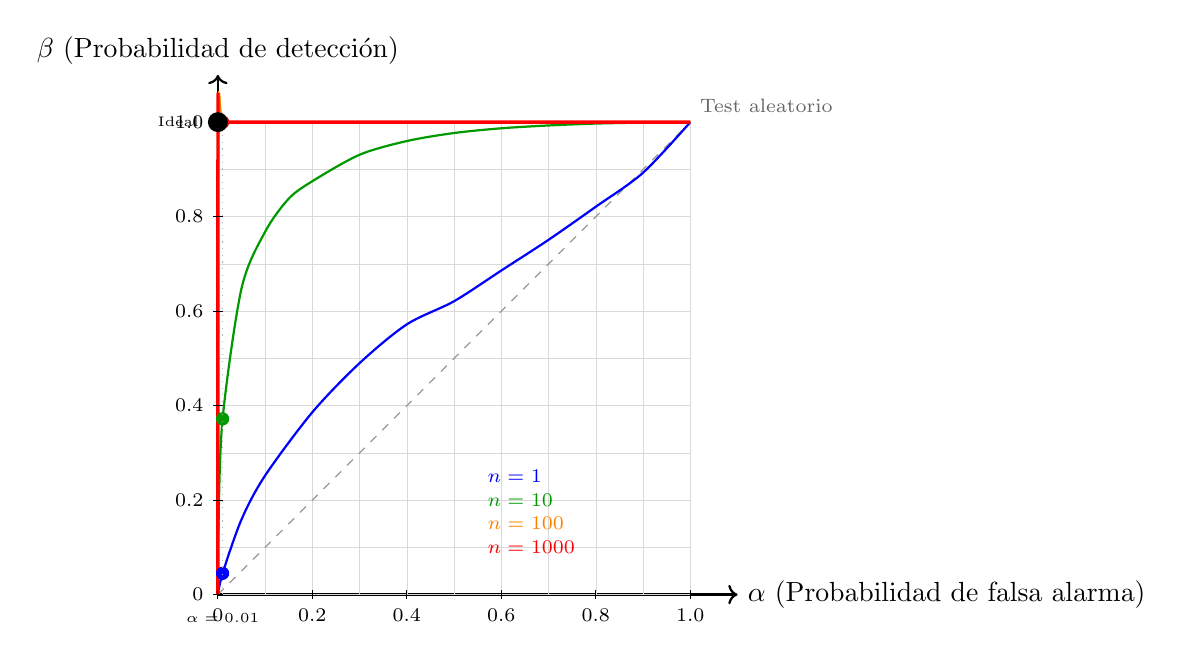
\begin{tikzpicture}[scale=6]
      % Ejes
      \draw[->, thick] (0,0) -- (1.1,0) node[right] {$\alpha$ (Probabilidad de falsa alarma)};
      \draw[->, thick] (0,0) -- (0,1.1) node[above] {$\beta$ (Probabilidad de detección)};
      
      % Grilla
      \draw[gray!30, very thin] (0,0) grid[step=0.1] (1,1);
      
      % Diagonal (test aleatorio sin información)
      \draw[black!40, dashed, thin] (0,0) -- (1,1) node[above right, font=\scriptsize, black!60] {Test aleatorio};
      
      % Curvas ROC (aproximadas usando curvas suaves)
      % n=1 (SNR=0.632) - curva cercana a la diagonal
      \draw[blue, thick, smooth] 
        plot coordinates {
          (0,0) (0.01,0.045) (0.05,0.159) (0.1,0.252) (0.2,0.386) 
          (0.3,0.490) (0.4,0.572) (0.5,0.621) (0.6,0.686) (0.7,0.751) 
          (0.8,0.821) (0.9,0.893) (1,1)
        };
      
      % n=10 (SNR=2.0) - curva intermedia
      \draw[green!60!black, thick, smooth] 
        plot coordinates {
          (0,0) (0.001,0.135) (0.01,0.372) (0.05,0.648) (0.1,0.768) 
          (0.15,0.838) (0.2,0.875) (0.3,0.931) (0.4,0.960) (0.5,0.977) 
          (0.6,0.987) (0.7,0.993) (0.8,0.997) (0.9,0.999) (1,1)
        };
      
      % n=100 (SNR=6.325) - curva muy cercana a la ideal
      \draw[orange, thick, smooth] 
        plot coordinates {
          (0,0) (0.001,0.999) (0.01,1.0) (0.05,1.0) (0.1,1.0) 
          (0.2,1.0) (0.5,1.0) (1,1)
        };
      
      % n=1000 (SNR=20.0) - prácticamente ideal
      \draw[red, very thick, smooth] 
        plot coordinates {
          (0,0) (0.0001,1.0) (0.001,1.0) (0.01,1.0) (0.1,1.0) (1,1)
        };
      
      % Punto de operación α=0.01 marcado
      \fill[blue] (0.01,0.045) circle (0.4pt);
      \fill[green!60!black] (0.01,0.372) circle (0.4pt);
      \fill[orange] (0.01,1.0) circle (0.4pt);
      \fill[red] (0.01,1.0) circle (0.4pt);
      
      % Línea vertical en α=0.01
      \draw[black!30, dotted] (0.01,0) -- (0.01,1);
      \node[below, font=\tiny] at (0.01,-0.02) {$\alpha=0.01$};
      
      % Leyenda
      \node[blue, font=\scriptsize, anchor=west] at (0.55, 0.25) {$n=1$};
      \node[green!60!black, font=\scriptsize, anchor=west] at (0.55, 0.20) {$n=10$};
      \node[orange, font=\scriptsize, anchor=west] at (0.55, 0.15) {$n=100$};
      \node[red, font=\scriptsize, anchor=west] at (0.55, 0.10) {$n=1000$};
      
      % Marcas en los ejes
      \foreach \x in {0, 0.2, 0.4, 0.6, 0.8, 1.0}
      \draw (\x,0.01) -- (\x,-0.01) node[below, font=\scriptsize] {\x};
      \foreach \y in {0, 0.2, 0.4, 0.6, 0.8, 1.0}
      \draw (0.01,\y) -- (-0.01,\y) node[left, font=\scriptsize] {\y};
      
      % Punto ideal (0,1)
      \fill[black] (0,1) circle (0.6pt);
      \node[left, font=\tiny] at (-0.02,1) {Ideal};
      
      \end{tikzpicture}
      \caption{Curvas ROC para detección de señalización antipodal con diferentes números de mediciones $n$. A medida que $n$ aumenta, las curvas se desplazan hacia el punto ideal (0,1), indicando mejor discriminación entre las hipótesis. La línea punteada vertical marca el punto de operación analizado en la parte 2.3 con $\alpha=0.01$.}
      \label{fig:curvas_roc_antipodal}
      \end{figure}
    \end{solution}
    %----------------------
    \question
    
    Considere un problema de detección binario $\Theta = \{0,1\}$ donde la variable aleatoria fuente de observación $X$ toma valores en la recta real $X = \mathbb{R}$ y sigue las estadísticas como función del parámetro $\theta$ dadas por:
    \begin{align}
    \theta = 0 &: X \sim \text{Uniforme}[0,1] \\
    \theta = 1 &: X \sim \text{Uniforme}[0,K]
    \end{align}
    con $K > 1$.
    
    \begin{parts}
        \part Determine la familia de test óptimos en el sentido del Lema de Neyman-Pearson. Considere solamente las familias de test óptimas de tamaño entre $[0,1]$.
        
        \part Fije un umbral $\tau \in \mathbb{R}$ y considere el siguiente test determinístico:
        \begin{equation}
        \pi_\tau(x) = 1 \text{ si } \log\frac{f_X(x|\theta=1)}{f_X(x|\theta=0)} \geq \tau
        \end{equation}
        
        y $\pi_\tau(x) = 0$ si la condición en (1.111) no se cumple. Determine las regiones de decisión de $\pi_\tau$, es decir los conjuntos $A_0^c = \pi_\tau^{-1}(\{0\})$ y $A_1^c = \pi_\tau^{-1}(\{1\})$. Exprese como función además dichas regiones como función de $\tau$. Identifique rangos concretos en el espacio de posibles valores de $\tau$.
        
        \part Del punto anterior, determine las expresiones para el poder y tamaño del test como función del valor de $\tau$. Recordar que:
        \begin{align}
        \alpha_{\pi_\tau} &= P_X(\pi_\tau(X) = 1 | \theta = 0) \\
        \beta_{\pi_\tau} &= P_X(\pi_\tau(X) = 1 | \theta = 1)
        \end{align}
        
        \part Determine la curva ROC. Es posible obtener la curva ROC completa (para todos los tamaños) con test determinísticos? Justifique.
        
        \part Vuelva al punto b) y d) y discuta que pasa con las regiones de decisión y la curva ROC si $K \to \infty$.
    \end{parts}
    %----------------------------
    \begin{solution}
      \subsection*{Resolución 3.1}
      
      Para determinar la familia de test óptimos según el Lema de Neyman-Pearson, necesitamos primero especificar las funciones de densidad de probabilidad bajo cada hipótesis.
      
      Bajo la hipótesis $\theta = 0$, tenemos $X \sim \text{Uniforme}[0,1]$:
      \begin{equation}
      f_X(x|\theta=0) = \begin{cases}
      1 & \text{si } x \in [0,1] \\
      0 & \text{en otro caso}
      \end{cases}
      \end{equation}
      
      Bajo la hipótesis $\theta = 1$, tenemos $X \sim \text{Uniforme}[0,K]$ con $K > 1$:
      \begin{equation}
      f_X(x|\theta=1) = \begin{cases}
      \frac{1}{K} & \text{si } x \in [0,K] \\
      0 & \text{en otro caso}
      \end{cases}
      \end{equation}
      
      El Lema de Neyman-Pearson establece que el test óptimo se basa en el cociente de verosimilitud:
      \begin{equation}
      L(x) = \frac{f_X(x|\theta=1)}{f_X(x|\theta=0)}
      \end{equation}
      
      Analicemos este cociente por regiones:
      
      \begin{itemize}
      \item \textbf{Para $x \in [0,1]$}: Ambas densidades son distintas de cero, por lo tanto:
      \begin{equation}
      L(x) = \frac{1/K}{1} = \frac{1}{K}
      \end{equation}
      
      \item \textbf{Para $x \in (1,K]$}: Solo la densidad bajo $\theta=1$ es distinta de cero, mientras que bajo $\theta=0$ es cero. En este caso:
      \begin{equation}
      L(x) = \frac{1/K}{0} = +\infty
      \end{equation}
      
      \item \textbf{Para $x \notin [0,K]$}: Ambas densidades son cero, por lo que el cociente no está definido (o se puede considerar que no aporta información).
      \end{itemize}
      
      El test óptimo de Neyman-Pearson tiene la forma:
      \begin{equation}
      \pi_\eta(x) = \begin{cases}
      1 & \text{si } L(x) > \eta \\
      \gamma_0 & \text{si } L(x) = \eta \\
      0 & \text{si } L(x) < \eta
      \end{cases}
      \end{equation}
      
      donde $\eta > 0$ es el umbral y $\gamma_0$ representa el valor esperado de la decisión cuando $L(x) = \eta$. Notemos que $\gamma_0$ toma valores en $[0,1]$, y en el contexto de detección binaria, este valor se interpreta como la probabilidad de decidir $\mathcal{H}_1$ mediante aleatorización.
      
      Dado que $K > 1$, tenemos que $\frac{1}{K} < 1$. Analicemos los diferentes casos según el valor de $\eta$:
      
      \begin{enumerate}
      \item \textbf{Si $\eta < \frac{1}{K}$}: Entonces $L(x) > \eta$ para todo $x \in [0,K]$. El test decide $\mathcal{H}_1$ en todo $[0,K]$:
      \begin{equation}
      \pi_\eta(x) = \begin{cases}
      1 & \text{si } x \in [0,K] \\
      0 & \text{si } x \notin [0,K]
      \end{cases}
      \end{equation}
      
      \item \textbf{Si $\eta = \frac{1}{K}$}: Entonces $L(x) = \eta$ para $x \in [0,1]$ y $L(x) > \eta$ para $x \in (1,K]$. Se requiere aleatorización en $[0,1]$:
      \begin{equation}
      \pi_\eta(x) = \begin{cases}
      1 & \text{si } x \in (1,K] \\
      \gamma_0 & \text{si } x \in [0,1] \\
      0 & \text{si } x \notin [0,K]
      \end{cases}
      \end{equation}
      
      \item \textbf{Si $\frac{1}{K} < \eta < +\infty$}: Entonces $L(x) < \eta$ para $x \in [0,1]$ y $L(x) > \eta$ para $x \in (1,K]$. El test decide:
      \begin{equation}
      \pi_\eta(x) = \begin{cases}
      1 & \text{si } x \in (1,K] \\
      0 & \text{si } x \in [0,1] \\
      0 & \text{si } x \notin [0,K]
      \end{cases}
      \end{equation}
      \end{enumerate}
      
      Por lo tanto, la familia de test óptimos de tamaño entre $[0,1]$ se caracteriza por:
      
      \begin{itemize}
      \item \textbf{Región determinística}: Siempre se decide $\mathcal{H}_1$ cuando $x \in (1,K]$ (ya que allí $L(x) = +\infty$)
      \item \textbf{Región de decisión variable}: En el intervalo $[0,1]$, la decisión depende del umbral $\eta$ y posiblemente de aleatorización
      \item \textbf{Parámetro de control}: El tamaño del test se controla mediante $\eta$ y $\gamma_0$. Con aleatorización, es posible alcanzar cualquier tamaño $\alpha \in [0,1]$ (intervalo cerrado).
      \end{itemize}
      
      La familia de test óptimos queda completamente caracterizada por el umbral $\eta \in (0, +\infty]$ y el valor esperado $\gamma_0 \in [0,1]$ cuando $\eta = \frac{1}{K}$, donde $\gamma_0$ representa la probabilidad de decidir $\mathcal{H}_1$ al aleatorizar en el intervalo $[0,1]$.
      
      \subsection*{Resolución 3.2}
      
      Consideremos el test determinístico dado por:
      \begin{equation}
      \pi_\tau(x) = 1 \text{ si } \log L(x) \geq \tau
      \end{equation}
      y $\pi_\tau(x) = 0$ en caso contrario.
      
      Primero, calculemos el logaritmo del cociente de verosimilitud en cada región:
      
      \begin{itemize}
      \item \textbf{Para $x \in [0,1]$}: 
      \begin{equation}
      \log L(x) = \log\left(\frac{1}{K}\right) = -\log K
      \end{equation}
      
      \item \textbf{Para $x \in (1,K]$}: 
      \begin{equation}
      \log L(x) = \log\left(+\infty\right) = +\infty
      \end{equation}
      
      \item \textbf{Para $x \notin [0,K]$}: El cociente no está definido o ambas densidades son cero.
      \end{itemize}
      
      La regla de decisión es: decidir $\mathcal{H}_1$ (es decir, $\pi_\tau(x) = 1$) si $\log L(x) \geq \tau$.
      
      Analicemos las regiones de decisión según el valor de $\tau$:
      
      \textbf{Caso 1: $\tau < -\log K$}
      
      En este caso:
      \begin{itemize}
      \item Para $x \in [0,1]$: $\log L(x) = -\log K$ y como $-\log K \geq \tau$, se decide $\mathcal{H}_1$
      \item Para $x \in (1,K]$: $\log L(x) = +\infty > \tau$, se decide $\mathcal{H}_1$
      \item Para $x \notin [0,K]$: No hay información, se decide $\mathcal{H}_0$ por defecto
      \end{itemize}
      
      Las regiones de decisión son:
      \begin{align}
      A_1^c &= \pi_\tau^{-1}(\{1\}) = [0,K] \\
      A_0^c &= \pi_\tau^{-1}(\{0\}) = \mathbb{R} \setminus [0,K]
      \end{align}
      
      \textbf{Caso 2: $\tau = -\log K$}
      
      En este caso:
      \begin{itemize}
      \item Para $x \in [0,1]$: $\log L(x) = -\log K = \tau$, se decide $\mathcal{H}_1$ (por la condición $\geq$)
      \item Para $x \in (1,K]$: $\log L(x) = +\infty > \tau$, se decide $\mathcal{H}_1$
      \item Para $x \notin [0,K]$: Se decide $\mathcal{H}_0$
      \end{itemize}
      
      Las regiones de decisión son:
      \begin{align}
      A_1^c &= \pi_\tau^{-1}(\{1\}) = [0,K] \\
      A_0^c &= \pi_\tau^{-1}(\{0\}) = \mathbb{R} \setminus [0,K]
      \end{align}
      
      \textbf{Caso 3: $-\log K < \tau < +\infty$}
      
      En este caso:
      \begin{itemize}
      \item Para $x \in [0,1]$: $\log L(x) = -\log K < \tau$, se decide $\mathcal{H}_0$
      \item Para $x \in (1,K]$: $\log L(x) = +\infty > \tau$, se decide $\mathcal{H}_1$
      \item Para $x \notin [0,K]$: Se decide $\mathcal{H}_0$
      \end{itemize}
      
      Las regiones de decisión son:
      \begin{align}
      A_1^c &= \pi_\tau^{-1}(\{1\}) = (1,K] \\
      A_0^c &= \pi_\tau^{-1}(\{0\}) = [0,1] \cup (\mathbb{R} \setminus [0,K])
      \end{align}
      
      \textbf{Caso 4: $\tau \geq +\infty$} (o $\tau$ muy grande)
      
      En este caso, ninguna observación finita satisface $\log L(x) \geq \tau$, por lo que:
      \begin{align}
      A_1^c &= \pi_\tau^{-1}(\{1\}) = \emptyset \\
      A_0^c &= \pi_\tau^{-1}(\{0\}) = \mathbb{R}
      \end{align}
      
      En resumen, las regiones de decisión como función de $\tau$ son:
      
      \begin{equation}
      A_1^c = \begin{cases}
      [0,K] & \text{si } \tau \leq -\log K \\
      (1,K] & \text{si } -\log K < \tau < +\infty \\
      \emptyset & \text{si } \tau \to +\infty
      \end{cases}
      \end{equation}
      
      \begin{equation}
      A_0^c = \begin{cases}
      \mathbb{R} \setminus [0,K] & \text{si } \tau \leq -\log K \\
      \mathbb{R} \setminus (1,K] & \text{si } -\log K < \tau < +\infty \\
      \mathbb{R} & \text{si } \tau \to +\infty
      \end{cases}
      \end{equation}
      
      Los rangos concretos de $\tau$ que definen comportamientos distintos son:
      \begin{itemize}
      \item $\tau \in (-\infty, -\log K]$: Test que decide $\mathcal{H}_1$ en todo $[0,K]$
      \item $\tau \in (-\log K, +\infty)$: Test que decide $\mathcal{H}_1$ solo en $(1,K]$
      \end{itemize}
      
      \subsection*{Resolución 3.3}
      
      Ahora determinaremos las expresiones para el tamaño ($\alpha_{\pi_\tau}$) y la potencia ($\beta_{\pi_\tau}$) del test como función de $\tau$.
      
      \textbf{Cálculo del tamaño del test:}
      
      El tamaño del test es la probabilidad de rechazar $\mathcal{H}_0$ cuando es verdadera:
      \begin{equation}
      \alpha_{\pi_\tau} = P_X(\pi_\tau(X) = 1 | \theta = 0) = P_X(X \in A_1^c | \theta = 0)
      \end{equation}
      
      Bajo $\theta = 0$, tenemos $X \sim \text{Uniforme}[0,1]$.
      
      \textbf{Caso 1: $\tau \leq -\log K$}
      
      En este caso, $A_1^c = [0,K]$. La probabilidad es:
      \begin{equation}
      \alpha_{\pi_\tau} = P_X(X \in [0,K] | \theta = 0) = P_X(X \in [0,1] | \theta = 0) = 1
      \end{equation}
      
      ya que bajo $\theta = 0$, $X$ solo toma valores en $[0,1] \subset [0,K]$.
      
      \textbf{Caso 2: $-\log K < \tau < +\infty$}
      
      En este caso, $A_1^c = (1,K]$. La probabilidad es:
      \begin{equation}
      \alpha_{\pi_\tau} = P_X(X \in (1,K] | \theta = 0) = 0
      \end{equation}
      
      ya que bajo $\theta = 0$, $X \in [0,1]$ y nunca puede estar en $(1,K]$.
      
      Por lo tanto:
      \begin{equation}
      \boxed{\alpha_{\pi_\tau} = \begin{cases}
      1 & \text{si } \tau \leq -\log K \\
      0 & \text{si } \tau > -\log K
      \end{cases}}
      \end{equation}
      
      \textbf{Cálculo de la potencia del test:}
      
      La potencia del test es la probabilidad de rechazar $\mathcal{H}_0$ cuando $\mathcal{H}_1$ es verdadera:
      \begin{equation}
      \beta_{\pi_\tau} = P_X(\pi_\tau(X) = 1 | \theta = 1) = P_X(X \in A_1^c | \theta = 1)
      \end{equation}
      
      Bajo $\theta = 1$, tenemos $X \sim \text{Uniforme}[0,K]$.
      
      \textbf{Caso 1: $\tau \leq -\log K$}
      
      En este caso, $A_1^c = [0,K]$. La probabilidad es:
      \begin{equation}
      \beta_{\pi_\tau} = P_X(X \in [0,K] | \theta = 1) = 1
      \end{equation}
      
      \textbf{Caso 2: $-\log K < \tau < +\infty$}
      
      En este caso, $A_1^c = (1,K]$. La probabilidad es:
      \begin{align}
      \beta_{\pi_\tau} &= P_X(X \in (1,K] | \theta = 1) \\
      &= \int_1^K \frac{1}{K} \, dx \\
      &= \frac{1}{K}(K - 1) \\
      &= \frac{K-1}{K} \\
      &= 1 - \frac{1}{K}
      \end{align}
      
      Por lo tanto:
      \begin{equation}
      \boxed{\beta_{\pi_\tau} = \begin{cases}
      1 & \text{si } \tau \leq -\log K \\
      1 - \frac{1}{K} & \text{si } \tau > -\log K
      \end{cases}}
      \end{equation}
      
      \textbf{Observaciones importantes:}
      
      \begin{itemize}
      \item El test solo tiene dos posibles comportamientos, determinados por si $\tau$ es mayor o menor/igual que $-\log K$.
      
      \item Cuando $\tau \leq -\log K$, el test es trivial: siempre decide $\mathcal{H}_1$ para cualquier observación en $[0,K]$, resultando en $\alpha = \beta = 1$.
      
      \item Cuando $\tau > -\log K$, el test decide $\mathcal{H}_1$ solo cuando $X \in (1,K]$. Este es el test no trivial interesante, con $\alpha = 0$ y $\beta = 1 - \frac{1}{K}$.
      
      \item Note que el test con $\tau > -\log K$ tiene tamaño cero ($\alpha = 0$), lo cual es óptimo desde el punto de vista de no cometer falsa alarma, pero tiene una potencia limitada de $1 - \frac{1}{K}$.
      
      \item A medida que $K$ aumenta, la potencia $\beta = 1 - \frac{1}{K}$ se acerca a 1, lo cual tiene sentido intuitivo: si $K$ es muy grande, la mayoría de las observaciones bajo $\mathcal{H}_1$ caerán en $(1,K]$.
      \end{itemize}
      
      \subsection*{Resolución 3.4}
      
      Para construir la curva ROC, debemos graficar $\beta$ versus $\alpha$ para todos los posibles tests.
      
      Del análisis anterior, vimos que los tests determinísticos solo pueden producir dos puntos en el espacio $(\alpha, \beta)$:
      
      \begin{enumerate}
      \item \textbf{Punto 1}: Cuando $\tau \leq -\log K$:
      \begin{equation}
      (\alpha, \beta) = (1, 1)
      \end{equation}
      
      Este es el test trivial que siempre decide $\mathcal{H}_1$.
      
      \item \textbf{Punto 2}: Cuando $\tau > -\log K$:
      \begin{equation}
      (\alpha, \beta) = \left(0, 1 - \frac{1}{K}\right)
      \end{equation}
      
      Este es el test que decide $\mathcal{H}_1$ solo cuando $X > 1$.
      \end{enumerate}
      
      Adicionalmente, siempre existe el test trivial que nunca decide $\mathcal{H}_1$:
      
      \begin{enumerate}
      \setcounter{enumi}{2}
      \item \textbf{Punto 3}: Test que siempre decide $\mathcal{H}_0$:
      \begin{equation}
      (\alpha, \beta) = (0, 0)
      \end{equation}
      \end{enumerate}
      
      \textbf{¿Es posible obtener la curva ROC completa con tests determinísticos?}
      
      \textbf{No}, no es posible obtener la curva ROC completa usando únicamente tests determinísticos. Los tests determinísticos solo producen tres puntos discretos:
      
      \begin{itemize}
      \item $(0, 0)$ - Test que nunca rechaza $\mathcal{H}_0$
      \item $\left(0, 1 - \frac{1}{K}\right)$ - Test óptimo no trivial
      \item $(1, 1)$ - Test que siempre rechaza $\mathcal{H}_0$
      \end{itemize}
      
      Para obtener la curva ROC completa, necesitamos tests aleatorizados. Consideremos un test aleatorizado general:
      
      \begin{equation}
      \pi_{\gamma_1}(x) = \begin{cases}
      1 & \text{si } x \in (1, K] \\
      \gamma_1 & \text{si } x \in [0,1] \\
      0 & \text{si } x \notin [0,K]
      \end{cases}
      \end{equation}
      
      donde $\gamma_1$ representa el valor esperado de la decisión (o probabilidad de decidir $\mathcal{H}_1$) cuando $x \in [0,1]$, con $\gamma_1 \in [0,1]$. En la implementación práctica de detección binaria, cuando $x \in [0,1]$ se aleatoriza: se decide $\mathcal{H}_1$ con probabilidad $\gamma_1$ y $\mathcal{H}_0$ con probabilidad $1-\gamma_1$.
      
      Para este test aleatorizado:
      
      \begin{align}
      \alpha &= P(X \in (1,K] | \theta=0) + \gamma_1 \cdot P(X \in [0,1] | \theta=0) \\
      &= 0 + \gamma_1 \cdot 1 \\
      &= \gamma_1
      \end{align}
      
      \begin{align}
      \beta &= P(X \in (1,K] | \theta=1) + \gamma_1 \cdot P(X \in [0,1] | \theta=1) \\
      &= \frac{K-1}{K} + \gamma_1 \cdot \frac{1}{K} \\
      &= 1 - \frac{1}{K} + \frac{\gamma_1}{K}
      \end{align}
      
      Eliminando $\gamma_1 = \alpha$ de la segunda ecuación:
      \begin{equation}
      \beta = 1 - \frac{1}{K} + \frac{\alpha}{K} = 1 - \frac{1-\alpha}{K}
      \end{equation}
      
      Esta es la ecuación de la curva ROC completa para $\alpha \in [0,1]$:
      
      \begin{equation}
      \boxed{\beta(\alpha) = 1 - \frac{1-\alpha}{K} = \frac{K-1+\alpha}{K}}
      \end{equation}
      
      Esta es una recta que conecta los puntos $(0, 1-\frac{1}{K})$ y $(1, 1)$.
      
      \textbf{Características de la curva ROC:}
      
      \begin{itemize}
      \item Es una función lineal de $\alpha$
      \item Tiene pendiente $\frac{1}{K}$
      \item Comienza en el punto $(0, 1-\frac{1}{K})$
      \item Termina en el punto $(1, 1)$
      \item No pasa por el origen $(0,0)$ a menos que se considere el test trivial que nunca rechaza
      \end{itemize}
      
      La curva ROC completa consiste en dos segmentos:
      
      \begin{enumerate}
      \item Segmento vertical desde $(0,0)$ hasta $(0, 1-\frac{1}{K})$: Se obtiene variando entre el test que nunca rechaza y el test determinístico óptimo
      \item Segmento lineal desde $(0, 1-\frac{1}{K})$ hasta $(1,1)$: Se obtiene con tests aleatorizados según la ecuación $\beta = 1 - \frac{1-\alpha}{K}$
      \end{enumerate}
      
      Por lo tanto, la respuesta es: \textbf{No es posible obtener la curva ROC completa con tests determinísticos}. Se requieren tests aleatorizados para llenar el segmento entre $(0, 1-\frac{1}{K})$ y $(1,1)$. Sin embargo, el test determinístico con $\tau > -\log K$ es óptimo en el sentido de que alcanza el punto con máxima potencia para tamaño cero.
      
      \subsection*{Resolución 3.5}
      
      Ahora analizaremos qué sucede con las regiones de decisión y la curva ROC cuando $K \to \infty$.
      
      \textbf{Análisis de las regiones de decisión (parte b):}
      
      Recordemos que las regiones de decisión son:
      
      Para $\tau \leq -\log K$:
      \begin{align}
      A_1^c &= [0,K] \\
      A_0^c &= \mathbb{R} \setminus [0,K]
      \end{align}
      
      Para $\tau > -\log K$:
      \begin{align}
      A_1^c &= (1,K] \\
      A_0^c &= \mathbb{R} \setminus (1,K]
      \end{align}
      
      Cuando $K \to \infty$:
      
      \begin{itemize}
      \item El umbral crítico $-\log K \to -\infty$. Esto significa que para cualquier valor finito de $\tau$, eventualmente tendremos $\tau > -\log K$ para $K$ suficientemente grande.
      
      \item Las regiones $[0,K]$ y $(1,K]$ se expanden hacia el infinito:
      \begin{align}
      \lim_{K \to \infty} [0,K] &= [0, \infty) \\
      \lim_{K \to \infty} (1,K] &= (1, \infty)
      \end{align}
      
      \item Para cualquier $\tau$ finito, el test con $K \to \infty$ decide:
      \begin{align}
      A_1^c &\to (1, \infty) \\
      A_0^c &\to (-\infty, 1]
      \end{align}
      
      \item La frontera de decisión se estabiliza en $x = 1$, independientemente del valor de $K$.
      \end{itemize}
      
      \textbf{Interpretación}: En el límite $K \to \infty$, el test óptimo determinístico tiene una forma simple: decide $\mathcal{H}_1$ si y solo si $x > 1$. Esta regla de decisión es intuitiva: bajo $\mathcal{H}_0$, $X \in [0,1]$ siempre, mientras que bajo $\mathcal{H}_1$ con $K$ muy grande, hay una probabilidad alta de observar $X > 1$.
      
      \textbf{Análisis de la curva ROC (parte d):}
      
      La curva ROC tiene la forma:
      \begin{equation}
      \beta(\alpha) = 1 - \frac{1-\alpha}{K}
      \end{equation}
      
      Cuando $K \to \infty$:
      \begin{equation}
      \lim_{K \to \infty} \beta(\alpha) = \lim_{K \to \infty} \left(1 - \frac{1-\alpha}{K}\right) = 1 - 0 = 1
      \end{equation}
      
      para todo $\alpha \in (0,1]$.
      
      Esto significa que la curva ROC converge a:
      
      \begin{equation}
      \beta(\alpha) = \begin{cases}
      0 & \text{si } \alpha = 0 \\
      1 & \text{si } \alpha \in (0, 1]
      \end{cases}
      \end{equation}
      
      En otras palabras, la curva ROC converge a una forma de "escalón" o función de Heaviside:
      
      \begin{itemize}
      \item Parte verticalmente desde $(0,0)$ hasta $(0,1)$
      \item Luego se extiende horizontalmente desde $(0,1)$ hasta $(1,1)$
      \end{itemize}
      
      \textbf{Interpretación y significado:}
      
      \begin{itemize}
      \item \textbf{Test casi perfecto}: Cuando $K \to \infty$, el problema de detección se vuelve "casi perfecto". Es posible alcanzar una potencia arbitrariamente cercana a 1 con un tamaño de test arbitrariamente pequeño.
      
      \item \textbf{Separación perfecta}: La razón es que, en el límite, las dos distribuciones se vuelven casi completamente separadas. Bajo $\mathcal{H}_0$, $X \in [0,1]$ con probabilidad 1. Bajo $\mathcal{H}_1$ con $K \to \infty$, la probabilidad de que $X > 1$ tiende a 1.
      
      \item \textbf{Región de soporte disjunto}: En el límite, tenemos:
      \begin{align}
      \text{Soporte de } f_0 &= [0,1] \\
      \lim_{K \to \infty} \text{Soporte de } f_1 &= [0, \infty)
      \end{align}
      
      La fracción del soporte de $f_1$ que se solapa con el soporte de $f_0$ es:
      \begin{equation}
      \frac{1}{K} \to 0 \text{ cuando } K \to \infty
      \end{equation}
      
      \item \textbf{Test óptimo simple}: El test óptimo en el límite es simplemente: decidir $\mathcal{H}_1$ si $X > 1$. Este test tiene:
      \begin{align}
      \alpha &= P(X > 1 | \theta = 0) = 0 \\
      \beta &= P(X > 1 | \theta = 1) = \lim_{K \to \infty} \frac{K-1}{K} = 1
      \end{align}
      
      \item \textbf{AUC perfecta}: El área bajo la curva ROC converge a:
      \begin{equation}
      \text{AUC} = \lim_{K \to \infty} \int_0^1 \beta(\alpha) \, d\alpha = \lim_{K \to \infty} \int_0^1 \left(1 - \frac{1-\alpha}{K}\right) d\alpha = 1
      \end{equation}
      
      Un AUC de 1 indica discriminación perfecta entre las dos hipótesis.
      \end{itemize}
      
      \textbf{Conclusión}: Cuando $K \to \infty$, el problema de detección se simplifica enormemente. Las dos distribuciones se separan casi completamente, haciendo posible una discriminación casi perfecta con un test determinístico simple (decidir $\mathcal{H}_1$ si $X > 1$). La curva ROC converge a la forma ideal de una función escalón, indicando rendimiento perfecto del detector.
      
    \end{solution}
\end{questions}
\end{document}